\section{Algorithms}\label{sec:algorithms}
This chapter describes how scalafmt formats Scala code.
We will see that scalafmt's design is inspired by ClangFormat and dartfmt.
However, we believe our design makes a valuable contribution in that it leverages functional programming principles to maximise code reuse and extensibility.

\subsection{Design}
Figure~\ref{fig:architecture} shows an architectural overview of scalafmt.
\begin{figure}
  \centering
  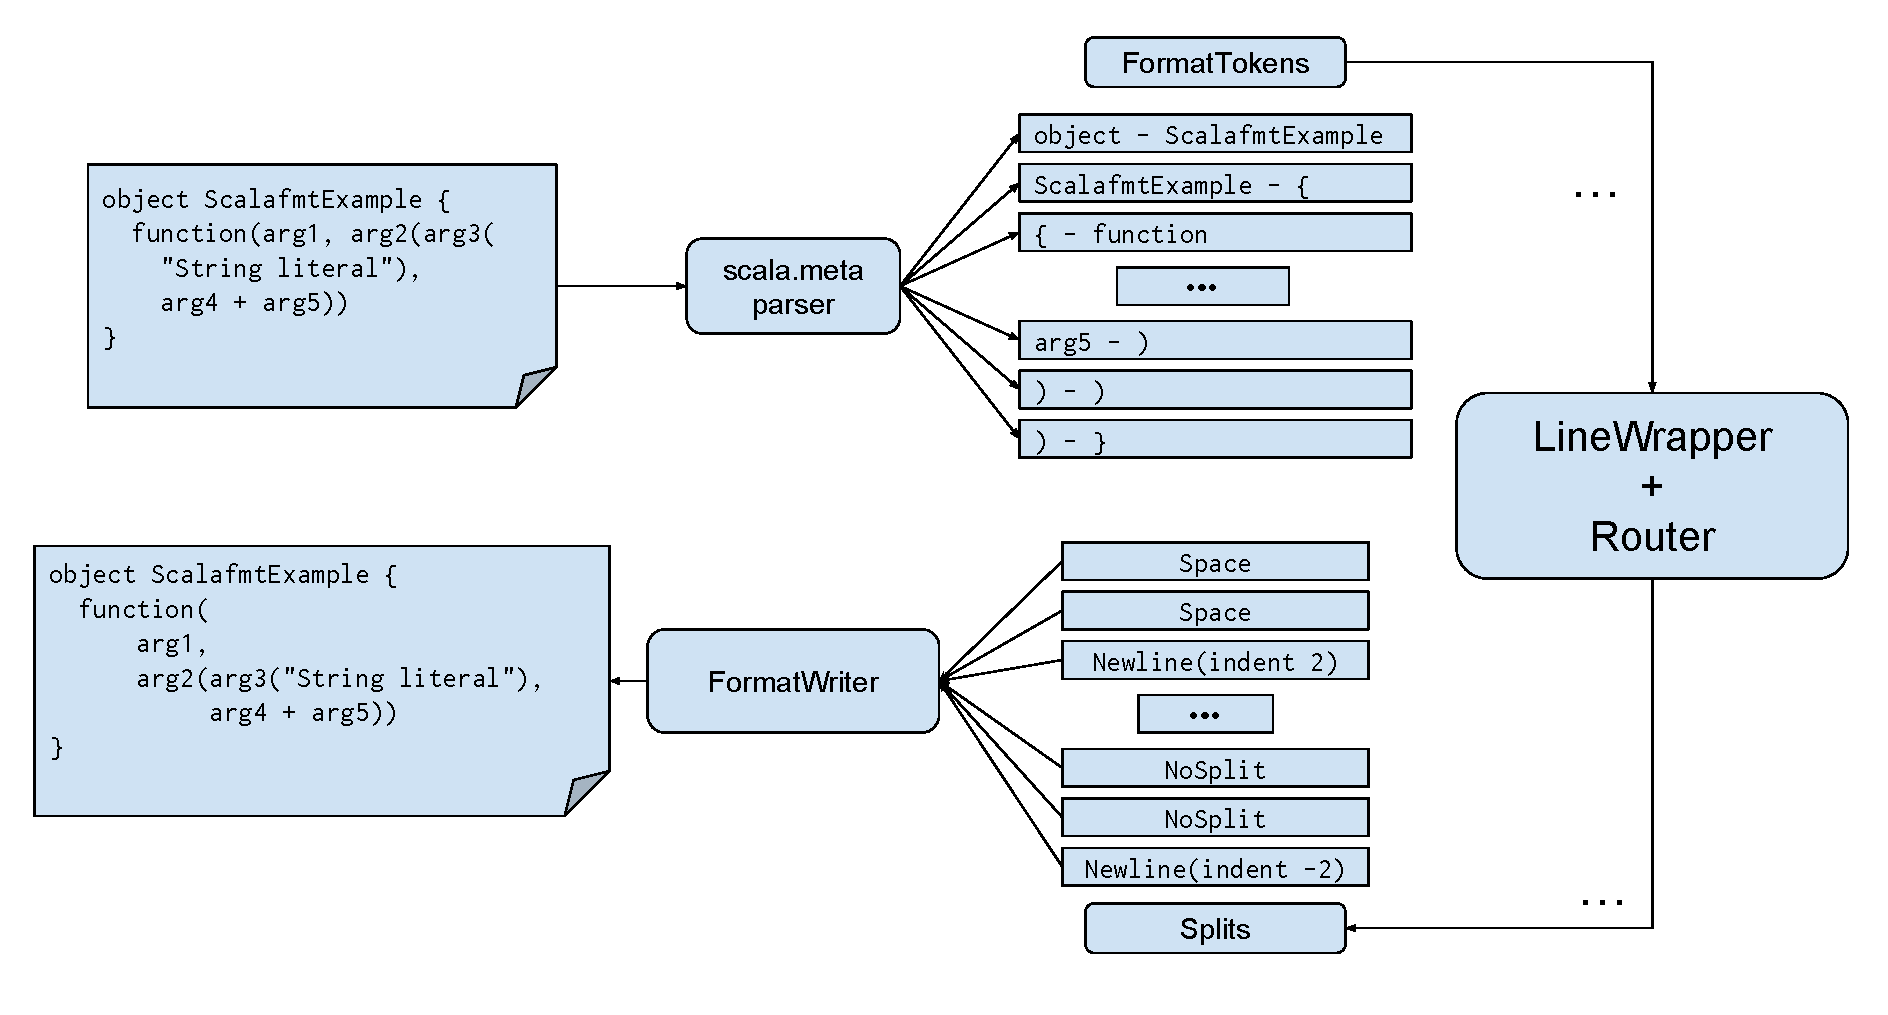
\includegraphics[width=\textwidth]{img/architechture.pdf}
  \caption{Scalafmt architecture}
  \label{fig:architecture}
\end{figure}
First, scalafmt parses a source file using scala.meta.
Next, we feed a sequence of \emph{FormatToken} data types into a \emph{LineWrapper}.
The LineWrapper uses a \emph{Router} to construct a weighted directed graph and run a best-first search to find an optimal formatting layout for the whole file.
Finally, the LineWrapper feeds a sequence of \emph{Split} data types into the \emph{FormatWriter}, which constructs a new reformatted source file.
The following sections explain these data types and abstractions in detail.

\subsection{Data structures}
Scalafmt leverages a few carefully designed data structure to allow an implementation that emphasizes correctness and maintainability.

\subsubsection{FormatToken}
A \emph{FormatToken} is a pair of two non-whitespace tokens.
Listing~\ref{lst:format_token} shows the definition of the FormatToken data type.
\lstinputlisting[label={lst:format_token}, float, caption=FormatToken definition]{code/format_token.scala}
As shown in the architecture overview in figure~\ref{fig:architecture}, each token except the beginning and end of file tokens appear twice in the sequence of FormatTokens: once as the \texttt{left} member and once as the \texttt{right} member.
In a nutshell, the job of the LineWrapper is to convert each FormatToken into a \emph{Split}

\subsubsection{Split}
A \emph{Split} represents a (possibly empty) whitespace character to be inserted between two non-whitespace tokens.
Listing~\ref{lst:split} shows the rather intricate definition of the Split data type\footnote{
  For clarity reasons, a few less important members have been removed from the actual Split definition.}.
\lstinputlisting[label={lst:split}, float, caption=Split definition]{code/split.scala}
The Split data type went through several generations of design before reaching its current structure.
Each member serves an important role.
The most important member of the Split type is the \emph{modification}.
A modification must be one of \texttt{NoSplit}, \texttt{Space} and \texttt{Newline}.
The \emph{cost} member represents the penalty for choosing this split.
The \emph{policy} member enables a Split to enforce a formatting layout over a region, explained in section~\ref{sec:policy}
The \emph{optimalToken} member enables an optimization discussed in section~\ref{sec:optimal}.
The \emph{indents} member adds a new layer of indentation, discussed in section~\ref{sec:indent}.
The \emph{line} member allows a powerful debugging technique explained in section~\ref{sec:line}.

\subsubsection{Indent}\label{sec:indent}
An \emph{Indent} describes indentation over a region of code.
\lstinputlisting[label={lst:indent}, float, caption=Indent definition]{code/indent.scala}
Listing~\ref{lst:indent} shows the definition of the Indent data type along with the algebraic data type \emph{Length}.
Length can either be a \texttt{Num(n)} where $n$ represents an explicit number of spaces to indent by or \texttt{StateColumn} which is a placeholder the number of spaces required to vertically align by the current column.
For example, given a scala.meta tree \texttt{expr}, the definition \texttt{Indent(Num(2), expr.tokens.last, inclusive=true)}
increases the indentation level by 2 spaces up to and including the last token of \texttt{expr}.
The expiration token is excluded for example in blocks wrapped by curly braces, since the closing curly brace should not be indented by 2 spaces.
The Length data type is required to allow memoization of Splits.

\subsection{LineWrapper}
\subsubsection{Router}\label{sec:router}
\subsubsection{Policy}\label{sec:policy}
\subsubsection{OptimalToken}\label{sec:optimal}
\subsubsection{State}
\subsection{Optimizations}
\subsubsection{dequeueOnNewStatements}
\subsubsection{recurseOnBlocks}
\subsubsection{escapeInPathologicalCases}
\subsubsection{escapeInPathologicalCases}
\subsubsection{pruneSlowStates}
\subsubsection{FormatWriter}
\begin{itemize}
  \item vertical alignment
  \item comment formatting
  \item stripMargin alignment
\end{itemize}
